\documentclass[11pt]{beamer}
\usetheme{Madrid}
\usepackage[utf8]{inputenc}
\usepackage{amsmath}

\usepackage{color}
\usepackage{listings}
\usepackage{mathtools}
\usepackage{tikz-cd}
\usepackage{adjustbox}

\definecolor{myblue}{rgb}{0,0,0.5}
\lstset{
	language=Python,
	tabsize=4,
	basicstyle=\footnotesize,
	keywordstyle=\bf\color{myblue},
	commentstyle=\it\color{gray},
	numbers=left,
	numbersep=3pt,
	numberstyle=\tiny\color{gray},
}

\author[\texttt{sebastiano.tronto@uni.lu}]{Sebastiano Tronto}
\title[Computational Complexity]%
{Why is my code slow?}
\logo{
\includegraphics[scale=0.1]{img/unilu.jpg}} 
%\institute{University of Luxembourg} 

\date{2021-05-21} 

\begin{document}

\begin{frame}
  \titlepage
\end{frame}

\begin{frame}{Computational Complexity}
	\begin{itemize}
		\item \textbf{Goal:}
		      estimate the running {\color{blue}time} of a program
		\item \textbf{How:}
		      count the {\color{blue}basic steps} that an
		      {\color{blue}algorithm} takes to complete
		\item \textbf{Why}:
		      find the \emph{bottleneck} of your program, make it faster
	\end{itemize}

	\vspace{0.5cm}
	Our analysis should not depend on the hardware
\end{frame}

\begin{frame}{Algorithm}
	\begin{definition}
		\emph{An algorithm is a sequence of {\color{blue}steps} needed to
		solve a {\color{blue}class of problems}. }
	\end{definition}

	\begin{definition}[alternative]
		\emph{An algorithm is a sequence of steps that takes
		an input satisfying certain conditions and produces an output
		satisfying other conditions.}
	\end{definition}
\end{frame}

\begin{frame}{Sorting a list}
	\begin{block}{Class of problems}
		Sort a list $L$ of numbers in increasing order.
	\end{block}

	\begin{block}{Algorithm}
		\begin{enumerate}
			\item Let $S$ be an empty list.
			\item Take an element from $L$ an insert it in $S$ in its correct
			      position.
			\item Repeat step $2$ until $L$ is empty.
			\item Return $S$.
		\end{enumerate}
	\end{block}
\end{frame}

\begin{frame}{Sorting a list}
\begin{itemize}
	\item It solves a \emph{class} of problems: works for any list
  	\item The specific steps to sort the list $[3,7,1]$ are not an algorithm
	\item Input conditions: must be a list of numbers
	\item Output conditions: same numbers in increasing order
\end{itemize}
\end{frame}

\begin{frame}{How to write an algorithm}
	\begin{itemize}
		\item \textbf{Human language}:
			\begin{itemize}
				\item Easy to understand
				\item Not precise
			\end{itemize}

		\vspace{0.3cm}
		\item \textbf{Computer code}:
			\begin{itemize}
				\item Can be executed by computers
				\item Precise
				\item From very low level (machine code) to high level
		      (Python, \dots)
		    \end{itemize}
	\end{itemize}

	%\vspace{0.5cm}
	%To what \emph{level of detail}?
\end{frame}

\begin{frame}{Basic steps}
	\begin{itemize}
		%\item Strictly speaking, only CPU instructions are \emph{basic}
		%\item In practice:%, we consider basic:
		%	\begin{itemize}
				\item Arithmetic operations $+,-,*,//,\%$
				\item Relational operations $==, !=, >, <,\dots$
				\item Memory access (read/write variable)
		%	\end{itemize}
	\end{itemize}

	\vspace{0.5cm}
	\textbf{Warning:}
		Depends on data type (integer, floating point, string,\dots)
	%\begin{itemize}
	%	\item Depends on data type (integer, floating point, string,\dots)
	%	\item There are non-basic instructions such as \texttt{sort()}
	%\end{itemize}
\end{frame}

\begin{frame}{Running time}
	\begin{itemize}
		\item Depends on computer power, programming language, compiler\dots
		%\item Not all basic steps are equal
		\item ``Big O'' notation: an algorithm runs in time $O(f(n))$ if, when
		      run with input of size $n$, it takes about $c\cdot f(n)$ steps
		\item Algorithm A is \emph{asymptotically faster} than algorithm B if
		      it is faster \textbf{for $n$ large enough}
		\item Rule of thumb: $10^7\sim10^9$ basic steps per second
	\end{itemize}
\end{frame}

\begin{frame}{Asymptotical analysis vs constant factors}
	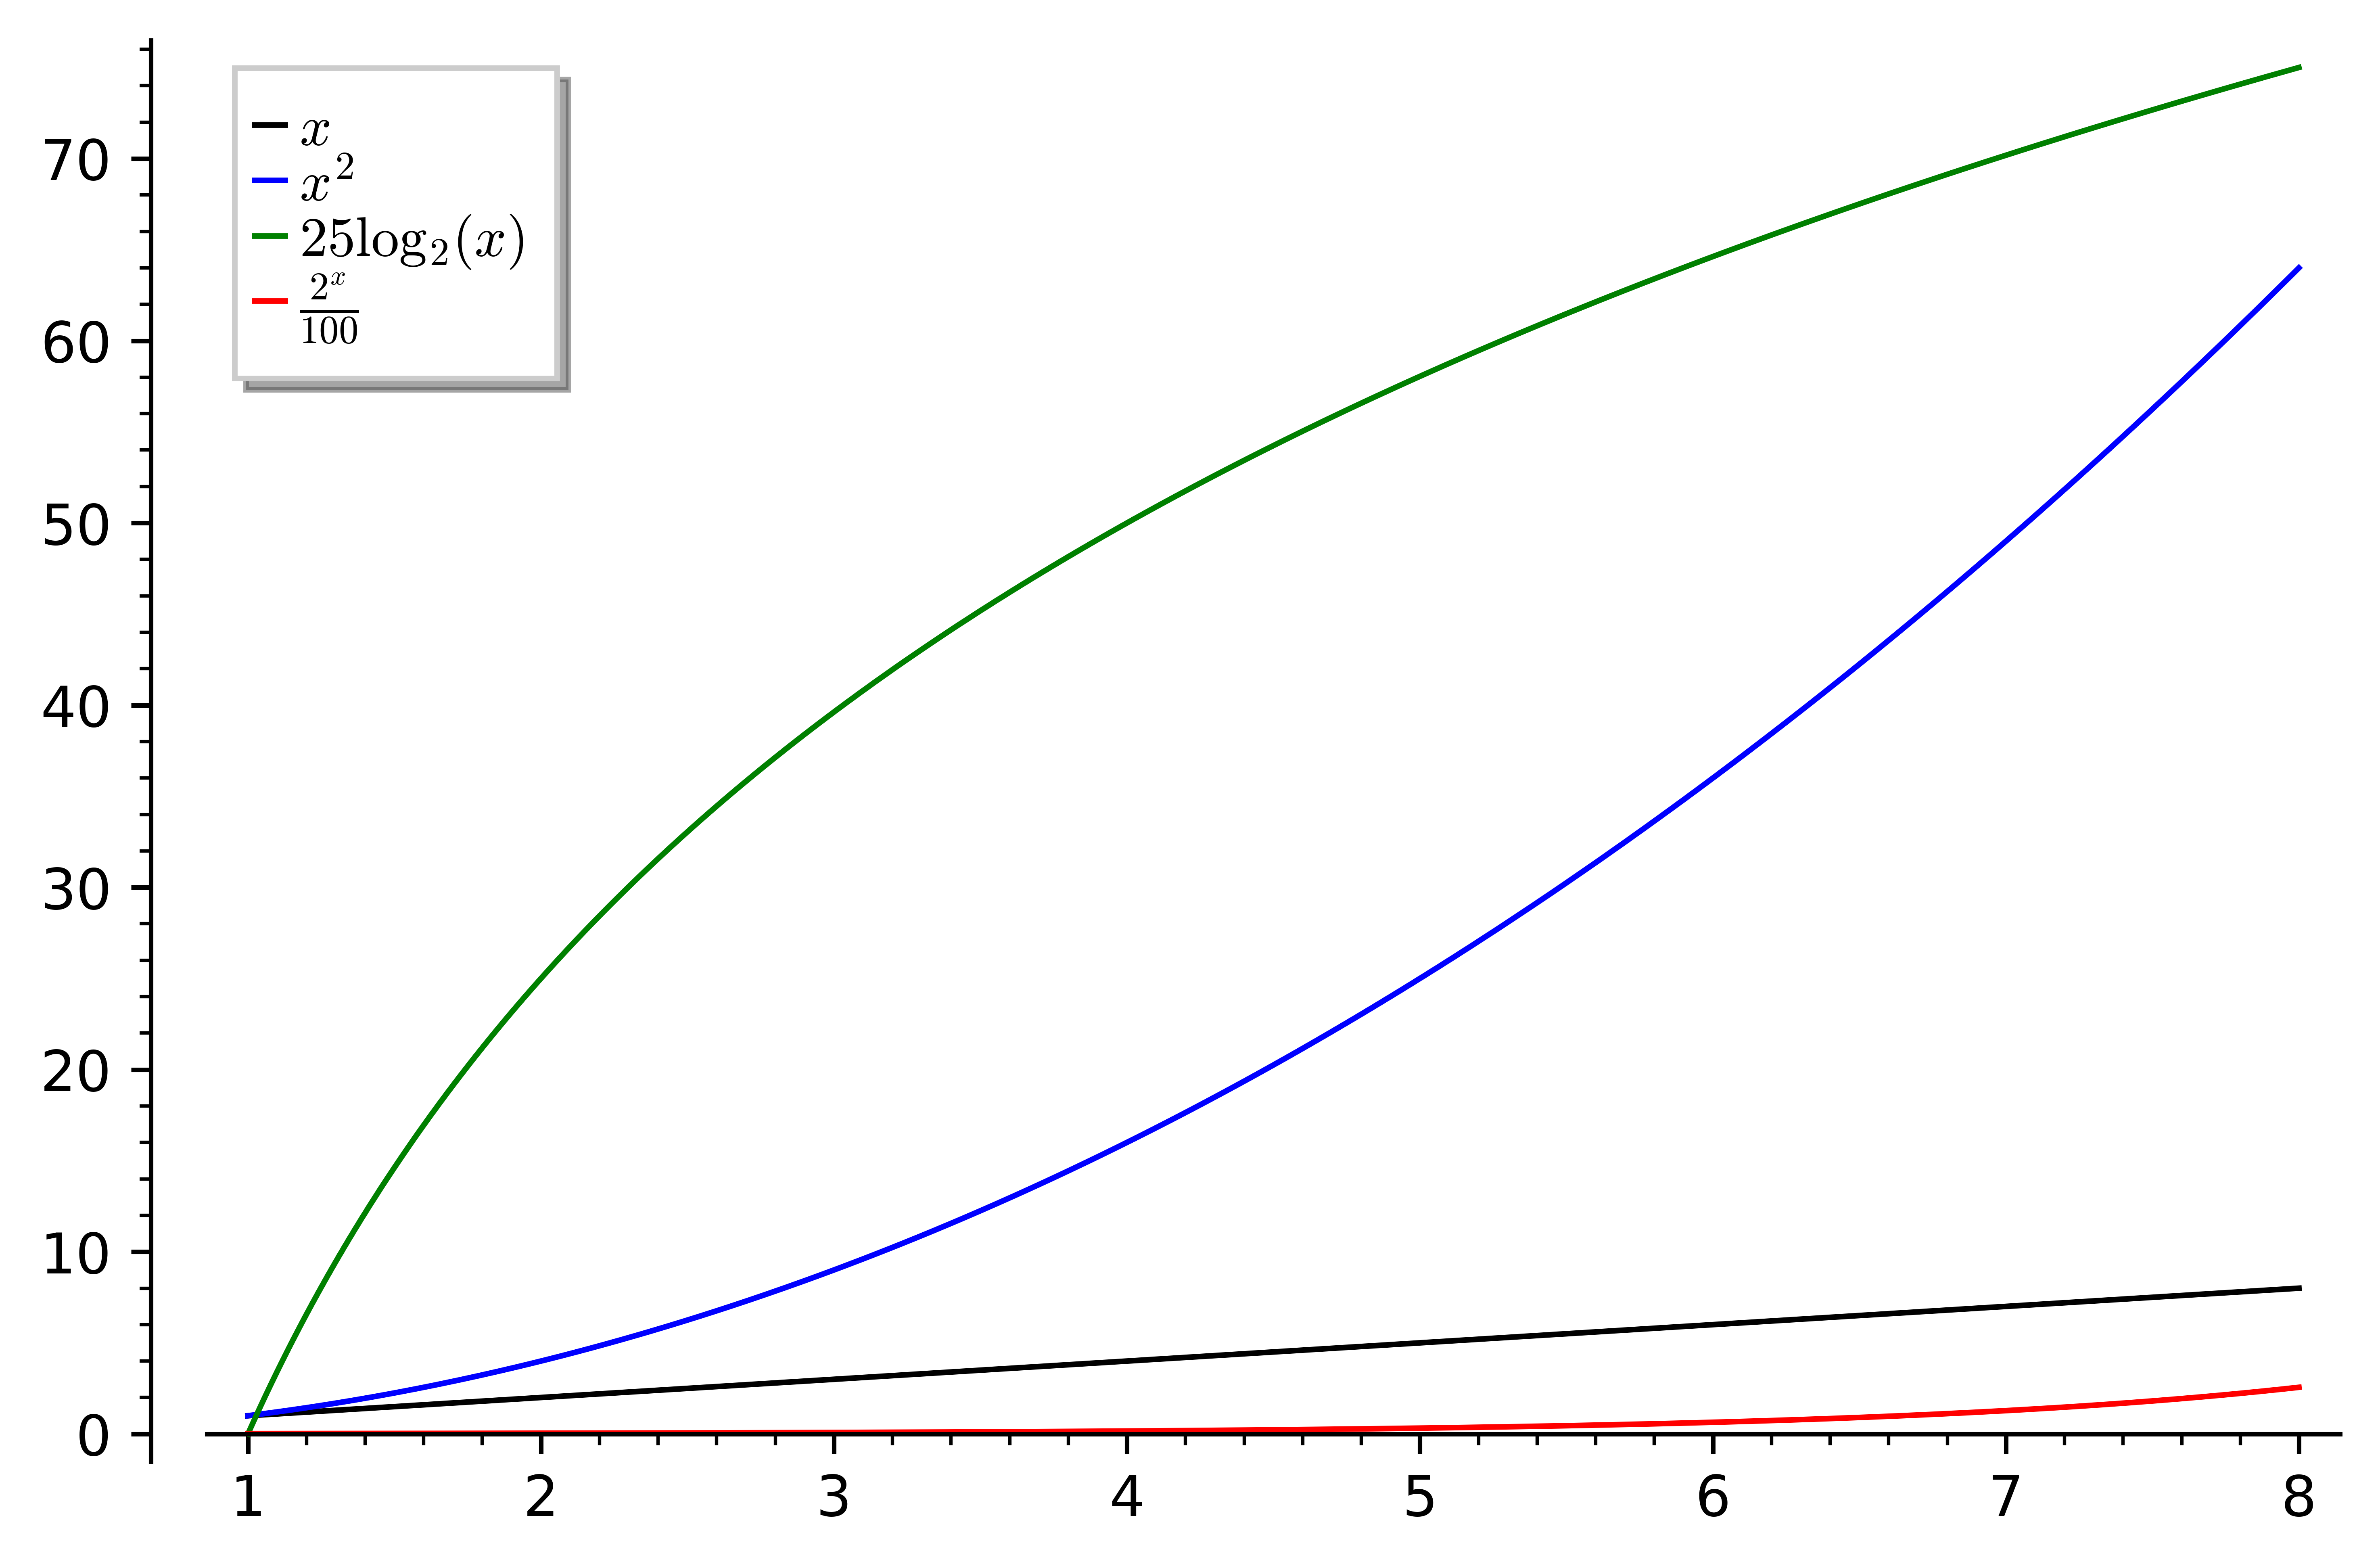
\includegraphics[scale=0.7]{img/plot1.png}
\end{frame}

\begin{frame}{Asymptotical analysis vs constant factors}
	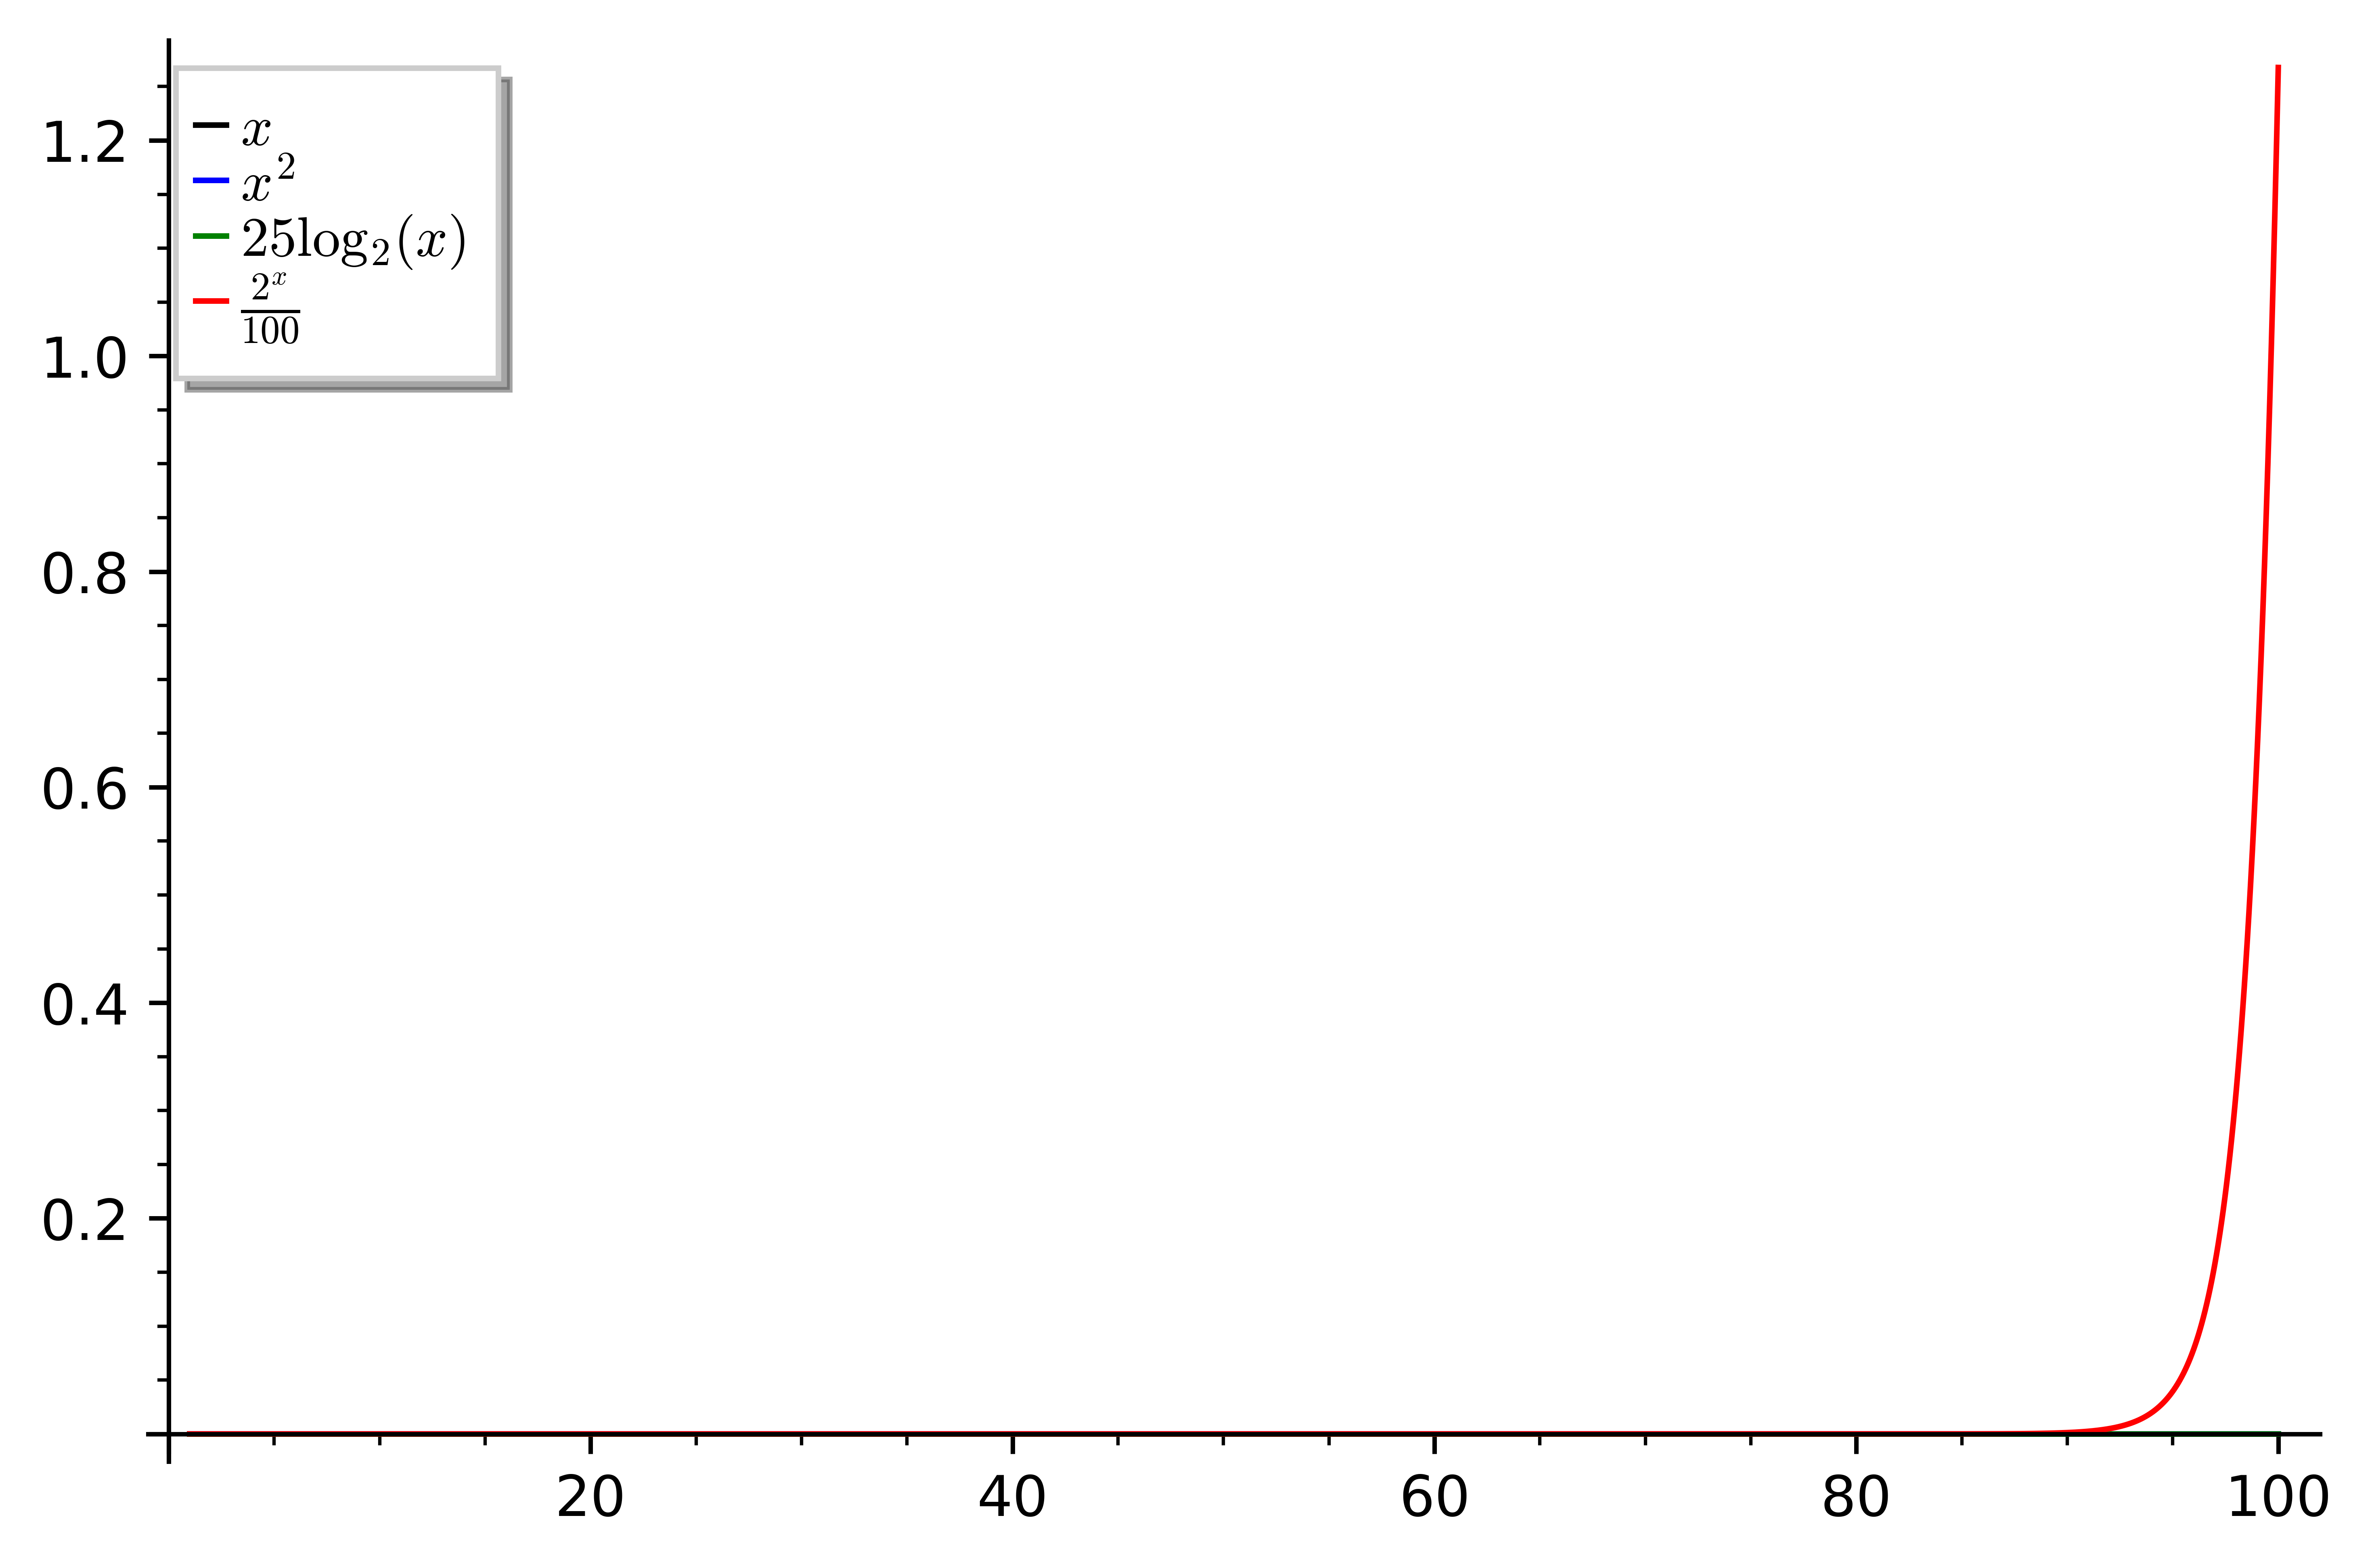
\includegraphics[scale=0.7]{img/plot2.png}
\end{frame}

\begin{frame}{Asymptotical analysis vs constant factors}
	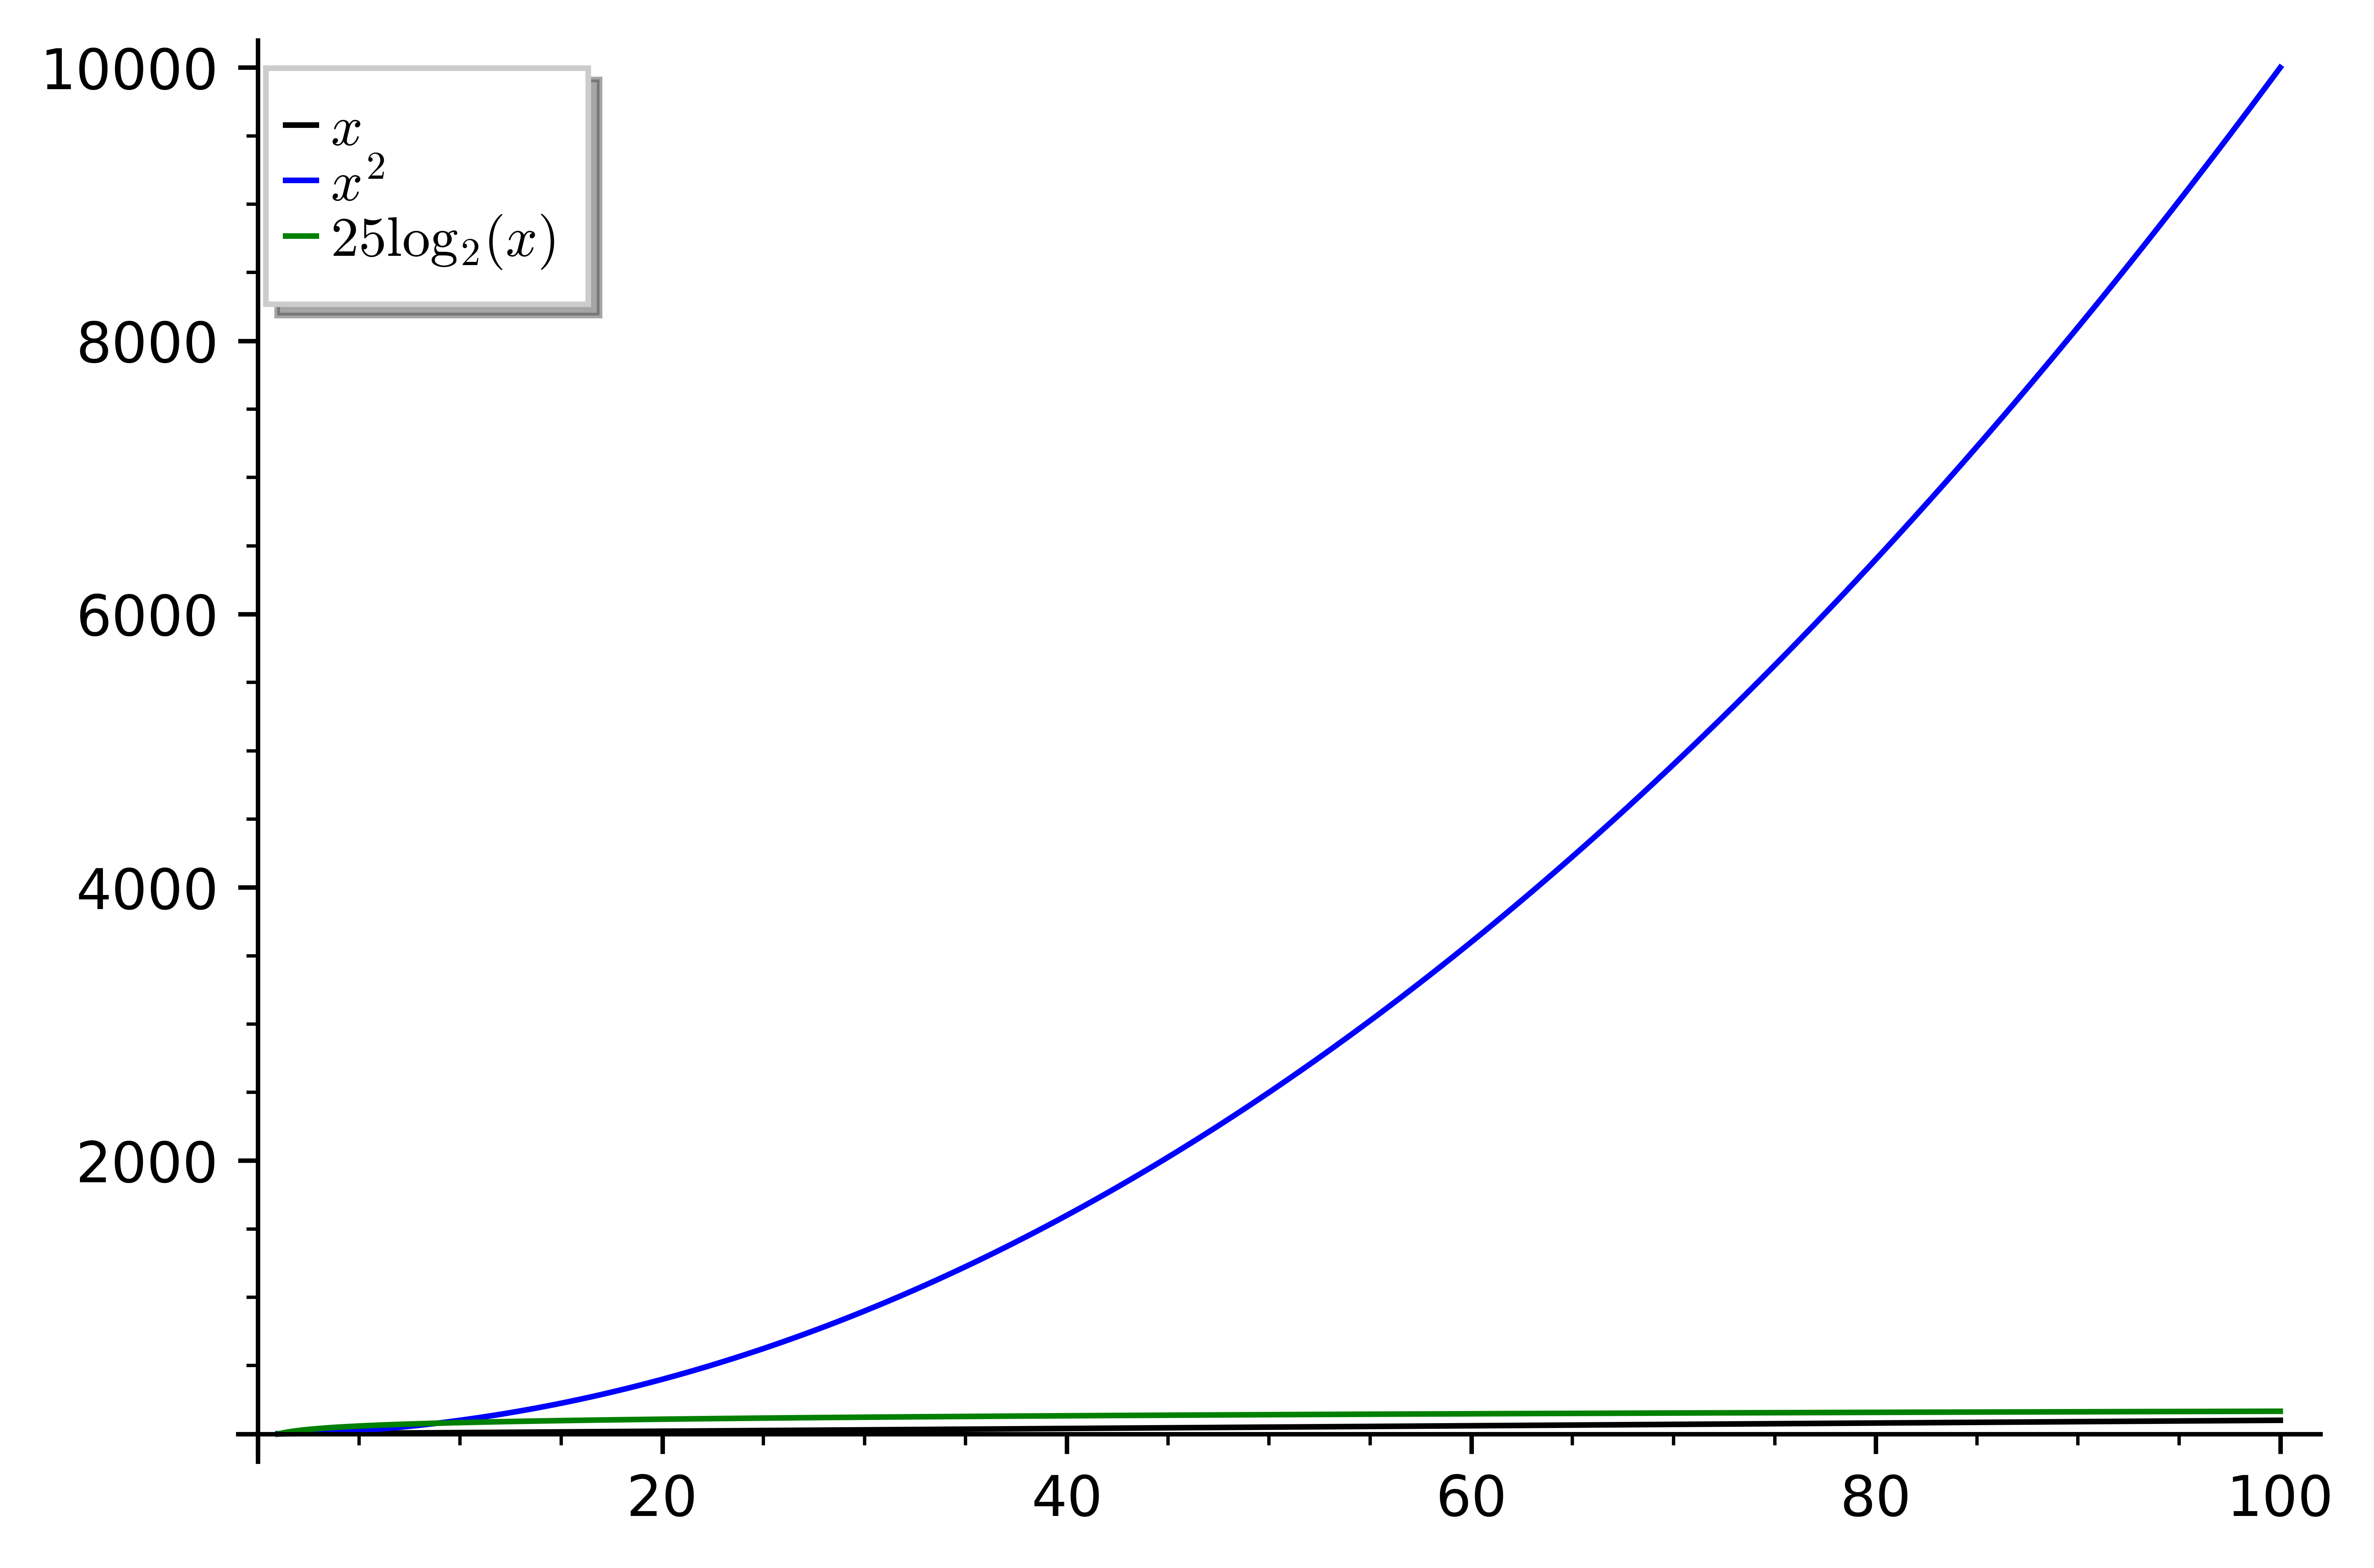
\includegraphics[scale=0.7]{img/plot3.png}
\end{frame}

\begin{frame}{Asymptotical analysis vs constant factors}
	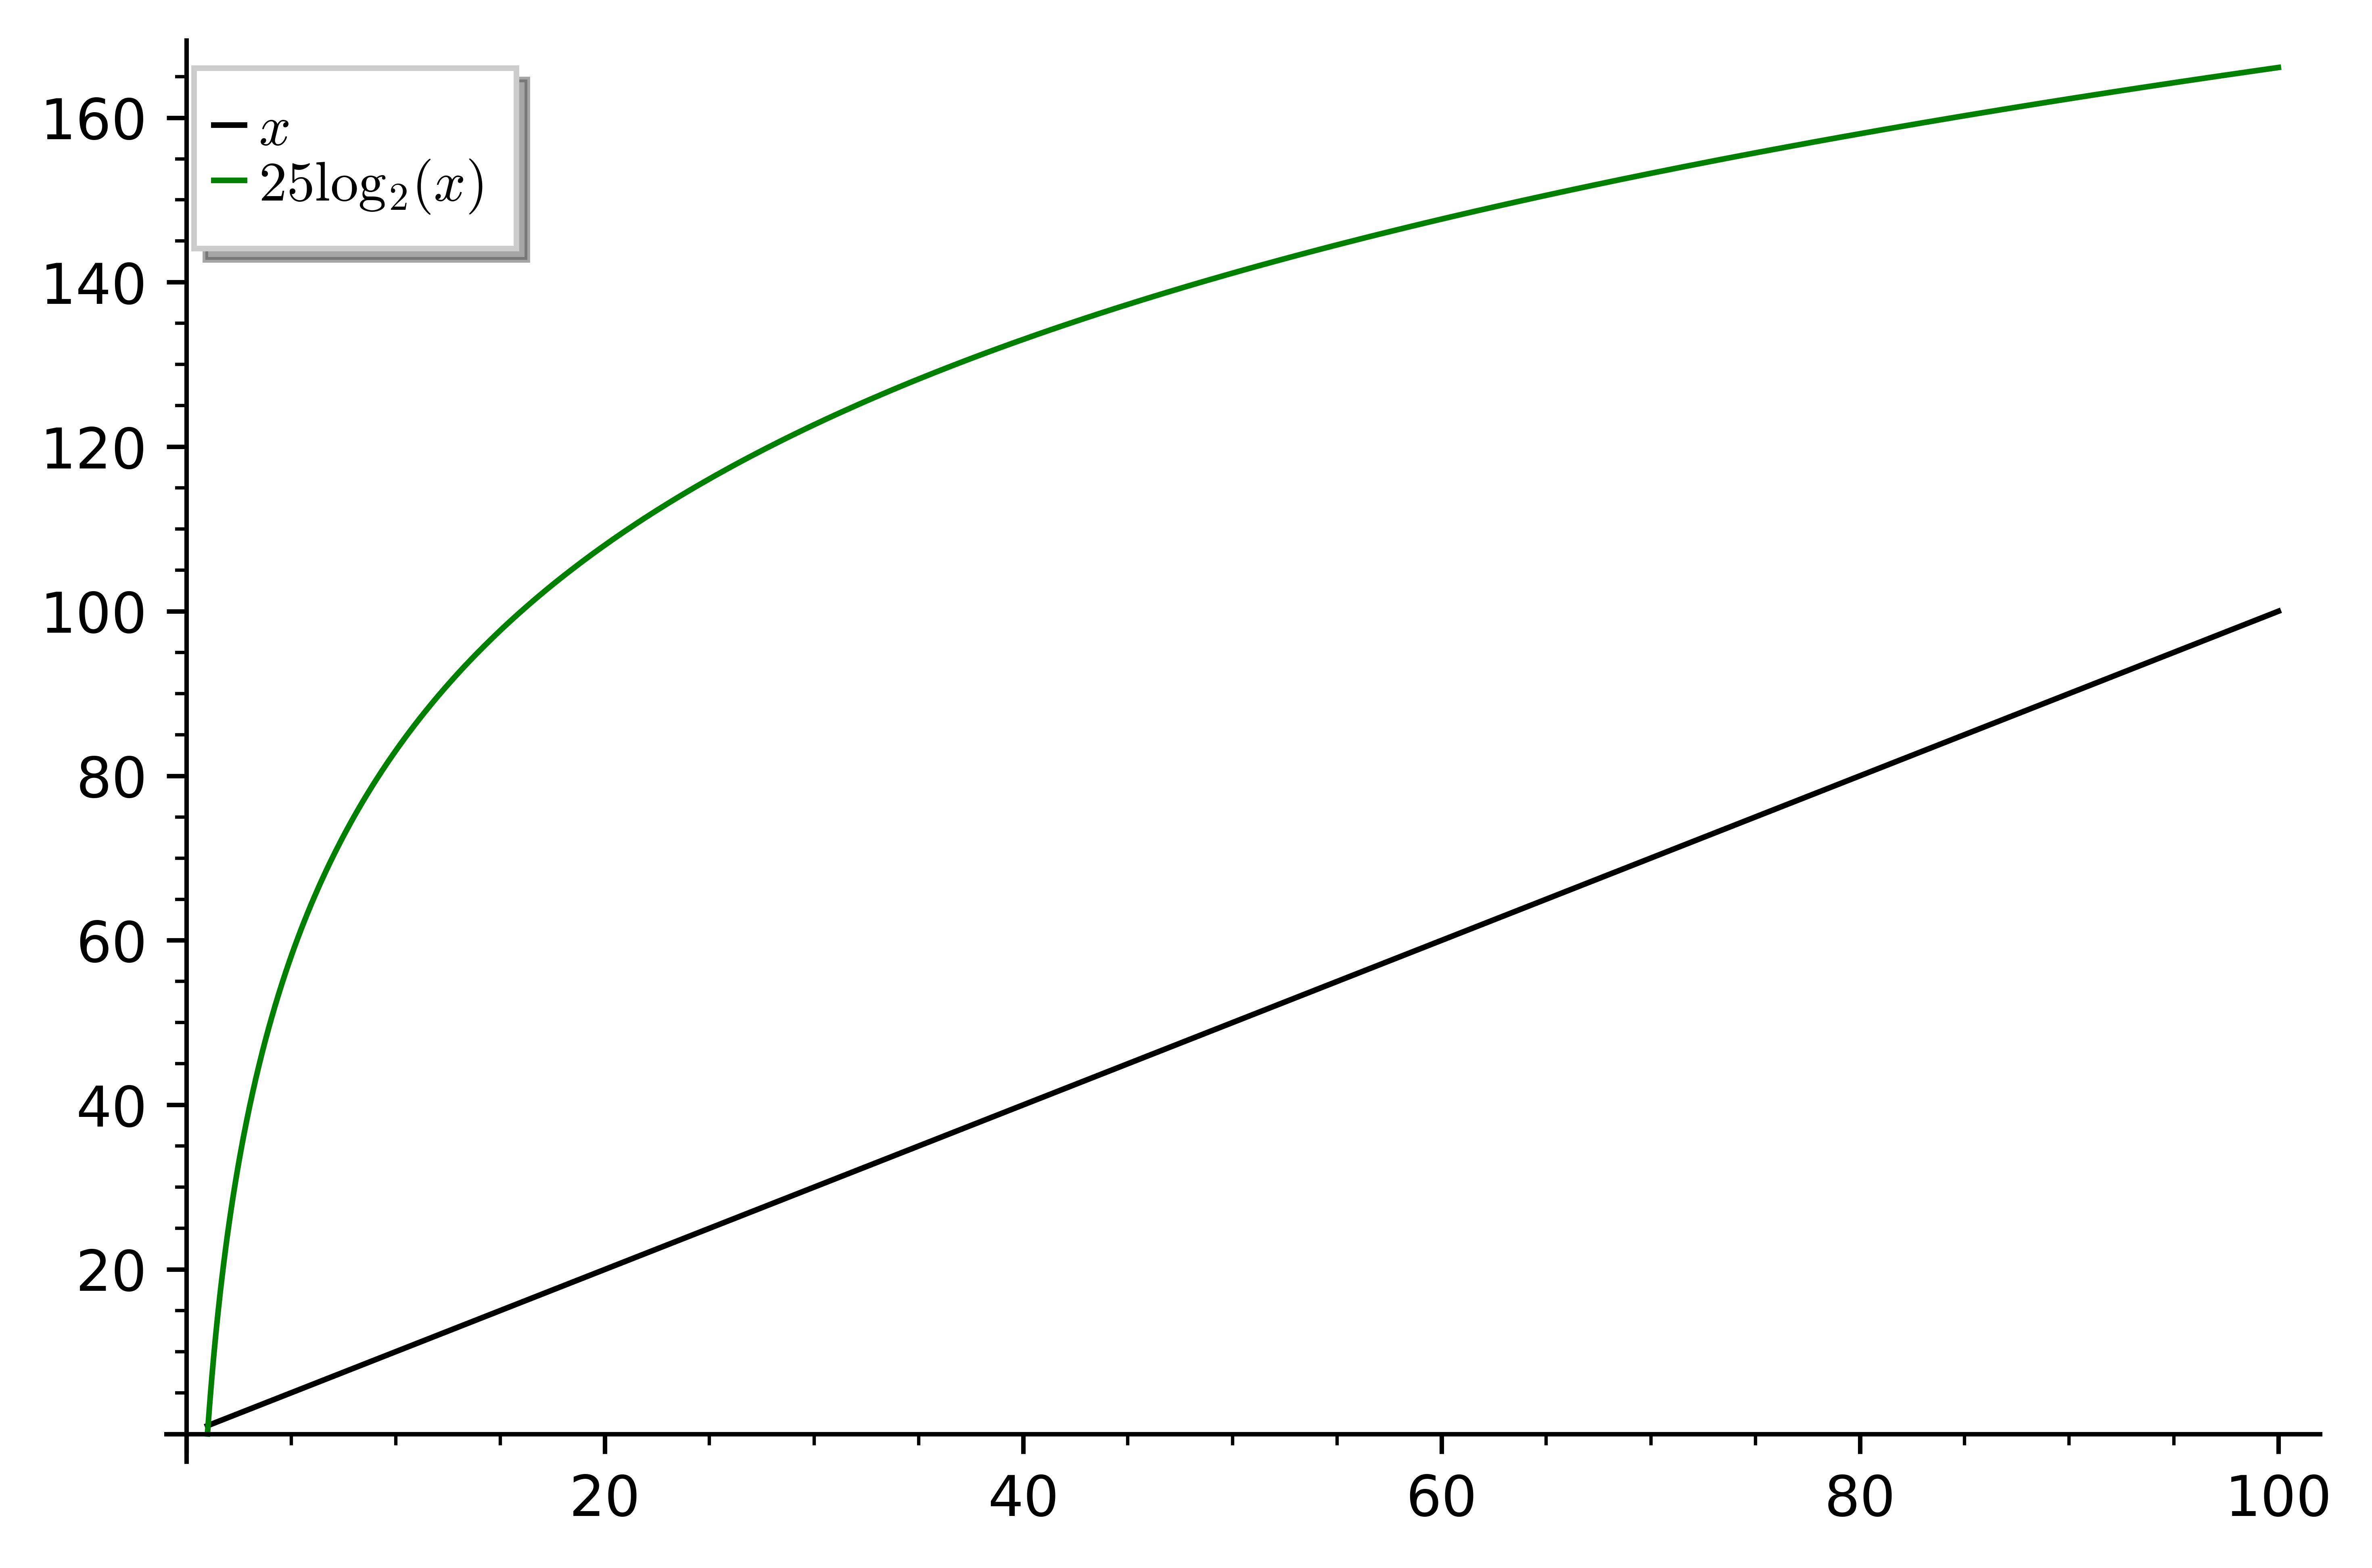
\includegraphics[scale=0.7]{img/plot4.png}
\end{frame}

\begin{frame}{Asymptotical analysis vs constant factors}
	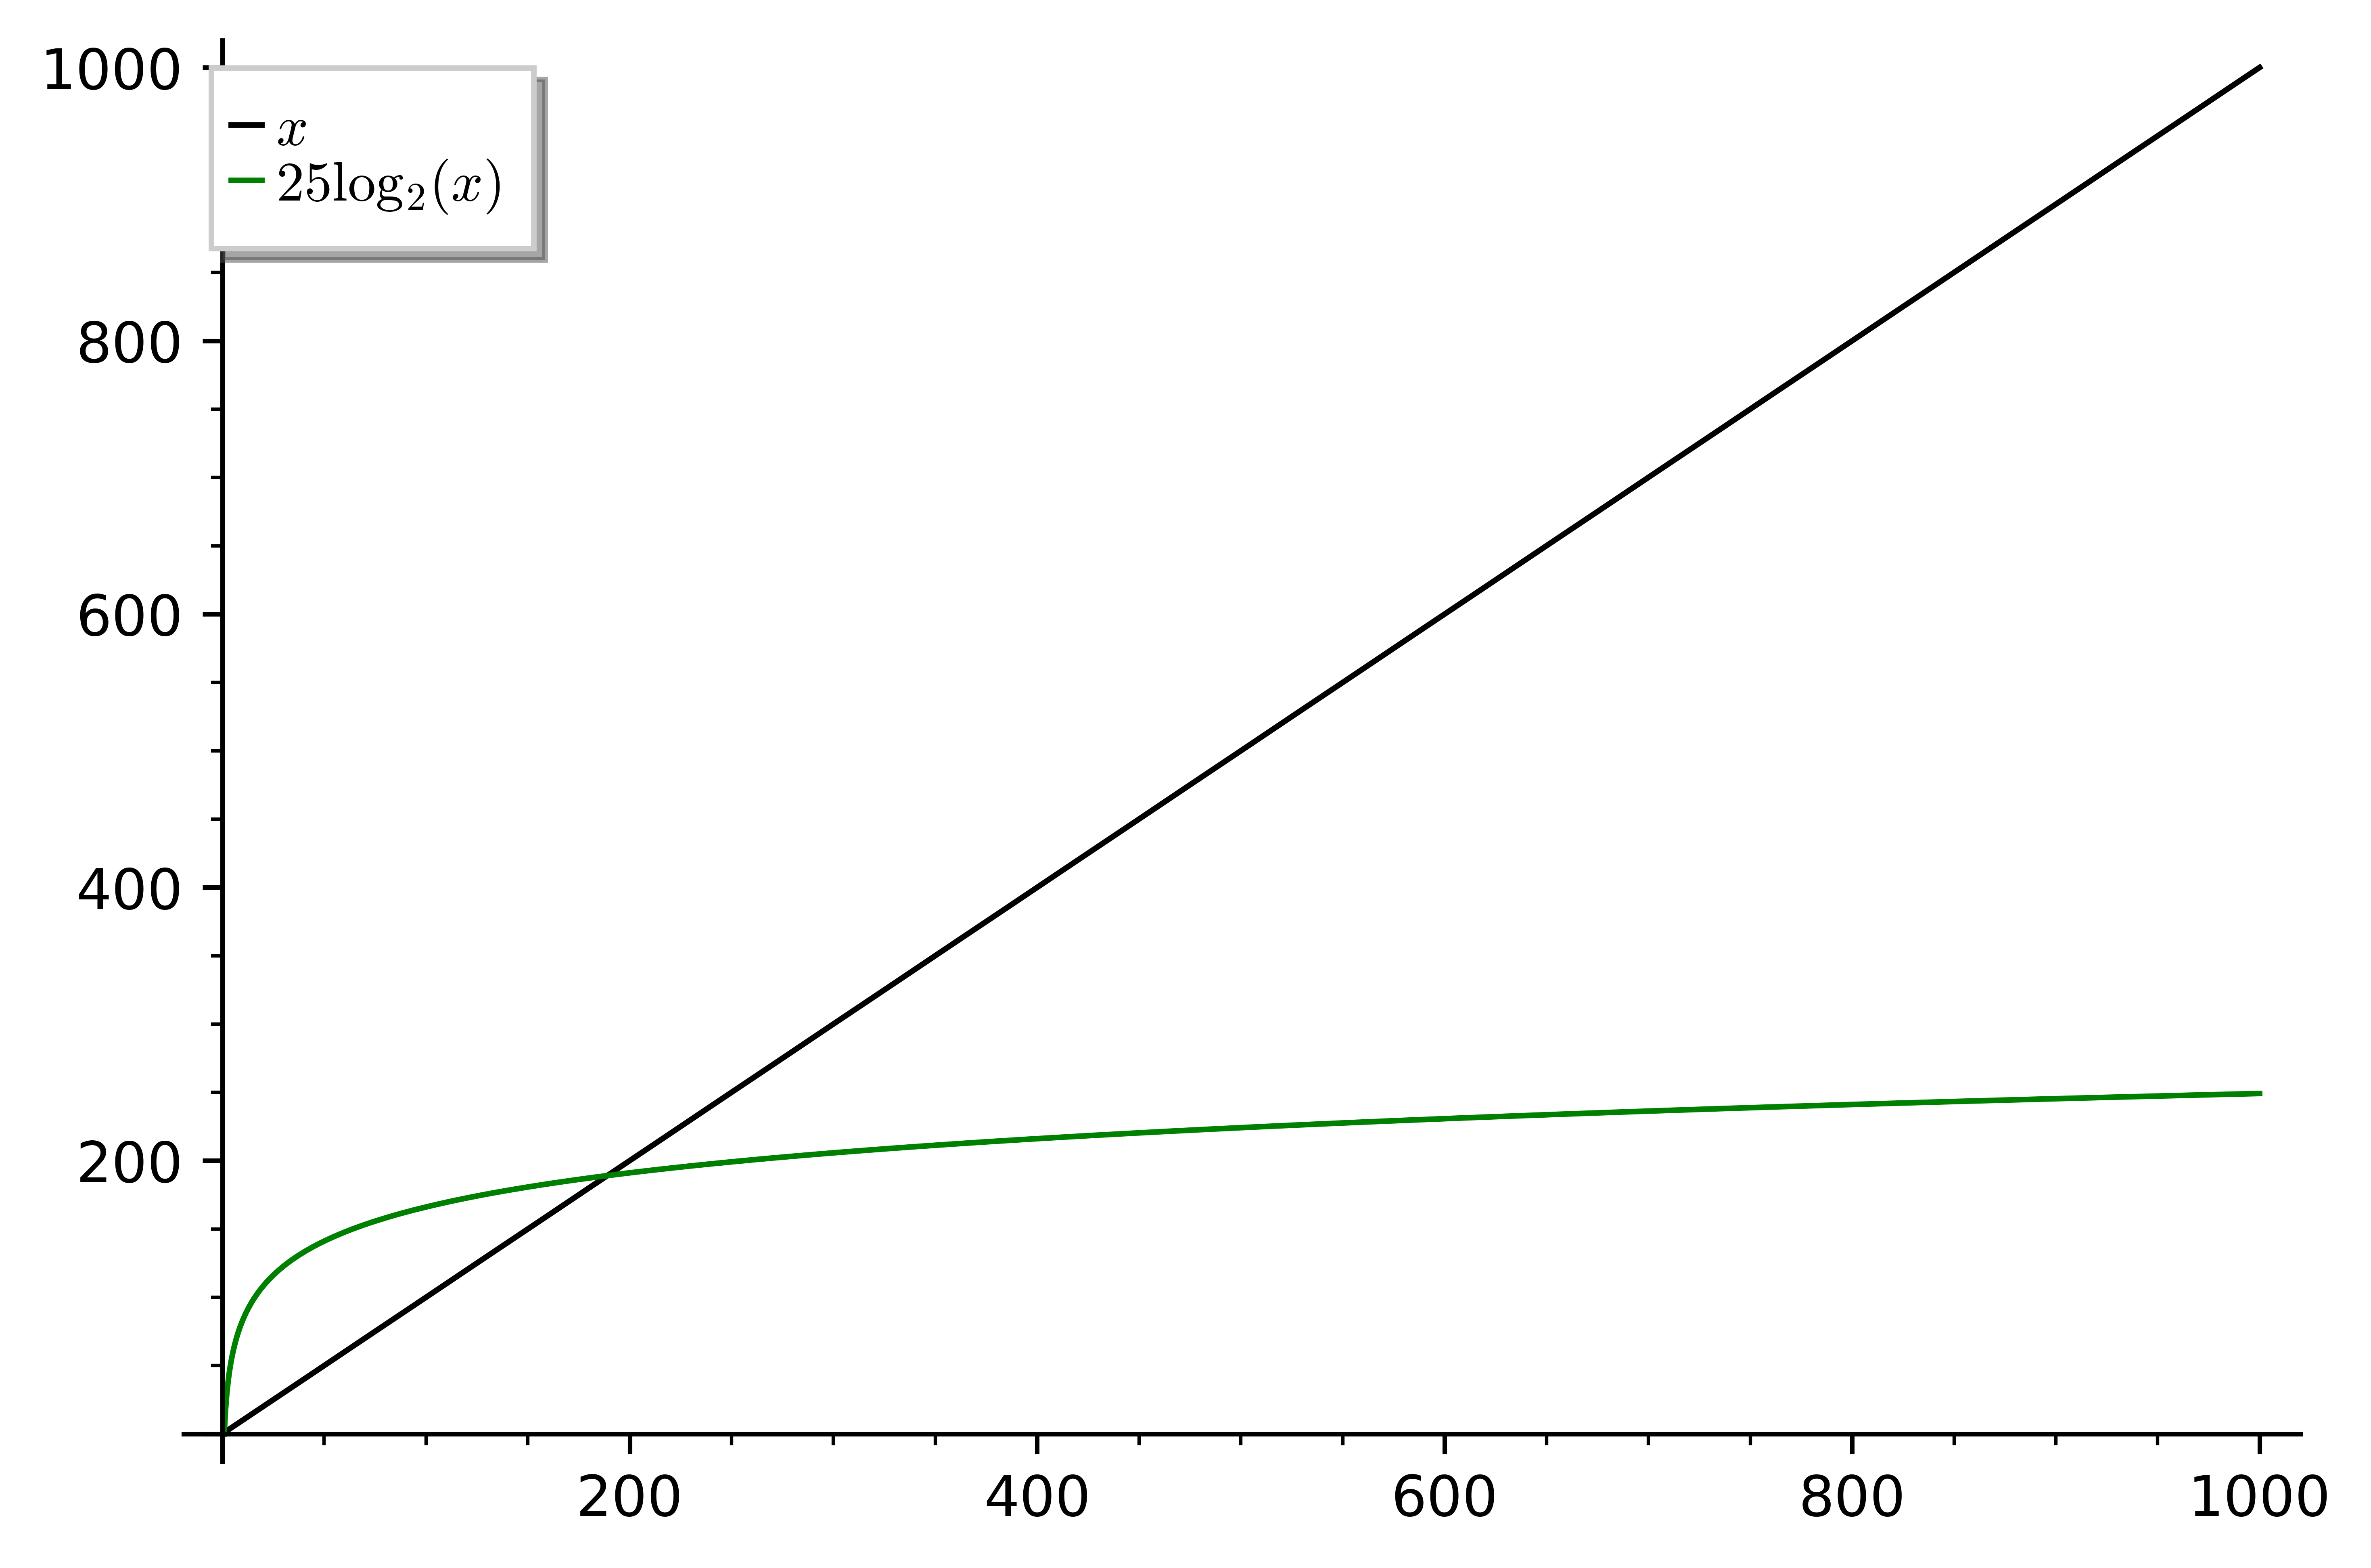
\includegraphics[scale=0.7]{img/plot5.png}
\end{frame}

%\begin{frame}{title}
%graphs here, uncomment
%\end{frame}

\begin{frame}{Basic complexity analysis}

	Easy things to do:

	\vspace{0.3cm}
	\begin{itemize}
		\item Check documentation for ``non-basic steps''
			\begin{itemize}
				\item Example: check Sage's \href{https://doc.sagemath.org/html/en/reference/rings\_standard/sage/rings/integer.html\#sage.rings.integer.Integer.is\_prime}{\texttt{is\_prime()}} (redirects to PARI \href{https://pari.math.u-bordeaux.fr/dochtml/html/Arithmetic\_functions.html\#se:isprime}{\texttt{isprime()}})
			\end{itemize}

	\vspace{0.3cm}
		\item Count nested loops
			\begin{itemize}
				\item How many times is a step repeated?
			\end{itemize}
	\end{itemize}
\end{frame}

{\setbeamertemplate{logo}{}
\begin{frame}[fragile]{Nested loops - matrix sum and product}
\begin{lstlisting}
def add(A, B):
	n = len(A)
	S = [[0] * n for i in range(n)]
	for i in range(0, n):
		for j in range(0, n):
			S[i][j] = A[i][j] + B[i][j]
	return S
\end{lstlisting}

\vspace{0.5cm}
\begin{lstlisting}
def prod(A, B):
	n = len(A)
	S = [[0] * n for i in range(n)]
	for i in range(0, n):
		for j in range(0, n):
			for k in range(0, n):
				S[i][j] = S[i][j] + A[i][k]*B[k][j]
	return S
\end{lstlisting}
\end{frame}
}

\begin{frame}{Nested loops - matrix sum and product}
	\begin{itemize}
		\item \texttt{add} is $O(n^2)$ (two loops)
		\item \texttt{prod} is $O(n^3)$ (three loops)
	\end{itemize}

	\vspace{0.3cm}
	\textbf{Fun fact:} there are faster algorithms for matrix multiplication,
	for example \href{https://en.wikipedia.org/wiki/Strassen_algorithm}%
	{Strassen's algorithm}.
\end{frame}

\begin{frame}[fragile]{Sorting a list}
\begin{lstlisting}
def correct_position(e, S):
	for i in range(0, len(S)):
		if S[i] > e:
			return i
	return len(S)

def sort_list(L):
	S = []
	for e in L:
		cp = correct_position(e, S)
		S.insert(cp, e)
	return S
\end{lstlisting}
\end{frame}

\begin{frame}{Sorting a list}
	\begin{itemize}
		\item Complexity of \texttt{correct\_position()}:
			\begin{itemize}
				%\item best case $O(1)$
				\item worst case $O($\texttt{len(S)}$)$
				\item average $O($\texttt{len(S)}$)$
			\end{itemize}

		\vspace{0.3cm}
		\item Complexity of \texttt{sort\_list} (here $n=$\texttt{len(L)}):
			\begin{align*}
				%\sum_{i=0}^{n-1} O(1) = O(n) && \text{best case}\\
				\sum_{i=0}^{n-1} O(i) = O(n^2)% && \text{average/worst}
			\end{align*}
			(it calls \texttt{correct\_position()} $n$ times).
	\end{itemize}
\end{frame}

\begin{frame}{Sorting a list}
	\begin{itemize}
		\item For which lists does the ``best case'' happen?
		\item For which lists does the ``worst case'' happen?
		\item How large can $n$ be for \texttt{sort\_list()} to run
		      in under a second?
	\end{itemize}
\end{frame}

\begin{frame}{Sorting a list}
	How to improve our code?
	\begin{itemize}
		\item Improve \texttt{correct\_position()}
		\item Take advantage of the fact that $S$ is always sorted
	\end{itemize}
\end{frame}

\begin{frame}{Binary search}
	\begin{block}{Algorithm}
		\textbf{Input:} a \emph{sorted} list $S$ and a value $e$.
		\begin{enumerate}
			\item If the list is empty, you have found the position of $e$
			\item Otherwise, compare $e$ to the middle element $m$ of $S$
			\begin{itemize}
				\item If $e<m$, repeat from (1) on the first half of $S$
				\item Otherwise, repeat from (1) on the second half of $S$
			\end{itemize}
		\end{enumerate}
	\end{block}
\end{frame}

\begin{frame}[fragile]{Binary search}
\begin{lstlisting}
# Return position of e in L
def binary_search(e, S, start, end):
	if start == end:
		return start
	midpoint = (end+start)//2
	if e < S[midpoint]:
		return binary_search(e, S, start, midpoint)
	else:
		return binary_search(e, S, midpoint+1, end)
\end{lstlisting}
\end{frame}

\begin{frame}{Binary search - example 1}
	Searching for \texttt{e}$=2$:
	\begin{align*}
	\only<1>{
		\underbrace{
			\overset{{\color{blue}
				\substack{\mathclap{\texttt{start}=0}\\\downarrow}}}{-2}
			\quad 0\quad 1\quad 3\quad 
			\overset{\substack{\mathclap{\texttt{midpoint}=4}\\\downarrow}}{5}
			\quad 6\quad 7\quad 9\quad 12
		}\quad
			\overset{{\color{red}
				\substack{\mathclap{\texttt{end}=9}\\\downarrow}}}{\phantom{0}}
	}
	\only<2>{
		\underbrace{
			\overset{{\color{blue}
				\substack{\mathclap{\texttt{start}=0}\\\downarrow}}}{-2}
			\quad 0\quad
			\overset{\substack{\mathclap{\texttt{midpoint}=2}\\\\\downarrow}}%
				{1}
			\quad 3
		}\quad
			\overset{{\color{red}
				\substack{\mathclap{\texttt{end}=4}\\\downarrow}}}{5}
		\quad 6\quad 7\quad 9\quad 12\quad \phantom{0}
	}
	\only<3>{
		-2\quad 0\quad 1\quad
		\underbrace{
			\overset{
				\substack{
					\mathclap{
						{\color{blue}\texttt{start}}=\texttt{midpoint}=3}\\\\
							{\color{blue}\downarrow}
				}
			}{3}
		} \quad
		\overset{{\color{red}
			\substack{\mathclap{\texttt{end}=4}\\\downarrow}}}{5}
		\quad 6\quad 7\quad 9\quad 12\quad \phantom{0}
	}
	\only<4>{
		-2\quad 0\quad 1\quad
		\overset{
			\substack{
				\mathclap{
					{\color{blue}\texttt{start}}=
						{\color{red}\texttt{end}}=3}\\\downarrow}}{3} 
		\quad 5 \quad 6\quad 7\quad 9\quad 12\quad \phantom{0}
	}
	\end{align*}
	\only<1>{{\color{blue}$e<5$}$\implies$ check left half}
	\only<2>{{\color{red}$e>1$}$\implies$ check right half}
	\only<3>{{\color{blue}$e<3$}$\implies$ check left half}
	\only<4>{\texttt{start}=\texttt{end}, done}
\end{frame}

\begin{frame}{Binary search - example 2}
	Searching for \texttt{e}$=11$:
	\begin{align*}
	\only<1>{
		\underbrace{
			\overset{{\color{blue}
				\substack{\mathclap{\texttt{start}=0}\\\downarrow}}}{-2}
			\quad 0\quad 1\quad 3\quad 
			\overset{\substack{\mathclap{\texttt{midpoint}=4}\\\downarrow}}{5}
			\quad 6\quad 7\quad 9\quad 12
		}\quad
			\overset{{\color{red}
				\substack{\mathclap{\texttt{end}=9}\\\downarrow}}}{\phantom{0}}
	}
	\only<2>{
		-2 \quad 0\quad 1 \quad 3 \quad 5 \quad
		\underbrace{
			\overset{{\color{blue}
				\substack{\mathclap{\texttt{start}=5}\\\downarrow}}}{6}
			\quad 7 \quad
			\overset{\substack{\mathclap{\texttt{midpoint}=7}\\\\\downarrow}}%
				{9}
			\quad 12
		}\quad
			\overset{{\color{red}
				\substack{\mathclap{\texttt{end}=9}\\\downarrow}}}{\phantom{0}}
	}
	\only<3>{
		-2\quad 0\quad 1\quad 3\quad 5\quad 6\quad 7\quad 9\quad
		\underbrace{
			\overset{
				\substack{
					\mathclap{
						{\color{blue}\texttt{start}}=\texttt{midpoint}=8}\\\\
							{\color{blue}\downarrow}
				}
			}{12}
		} \quad
		\overset{{\color{red}
			\substack{\mathclap{\texttt{end}=9}\\\downarrow}}}{\phantom{0}}
	}
	\only<4>{
		-2\quad 0\quad 1\quad 3\quad 5\quad 6\quad 7\quad 9\quad
		\overset{
			\substack{
				\mathclap{
					{\color{blue}\texttt{start}}=
						{\color{red}\texttt{end}}=8}\\\downarrow}}{12} 
	}
	\end{align*}
	\only<1>{{\color{red}$e>5$}$\implies$ check right half}
	\only<2>{{\color{red}$e>9$}$\implies$ check right half}
	\only<3>{{\color{blue}$e<11$}$\implies$ check left half}
	\only<4>{\texttt{start}=\texttt{end}, done}
\end{frame}

\begin{frame}{Binary search}
	\begin{itemize}
		\item Works only if the list is sorted
		\item Complexity $O(\log_2(n))$: at every step we cut the list in half
		\item Recursive, \emph{divide et impera}
	\end{itemize}
\end{frame}

\begin{frame}[fragile]{Sorting a list - binary search version}
\begin{lstlisting}
def sort_list(L):
	S = []
	for e in L:
		cp = binary_search(e, S, 0, len(S)) # This changed
		S.insert(cp, e)
	return S
\end{lstlisting}
	\vspace{0.3cm}
	\begin{itemize}
		\item Complexity: \[\sum_{i=0}^{n-1} O(\log_2(i)) = O(n\log_2(n))\]\\
			(it calls \texttt{binary\_search} $n$ times).
	\end{itemize}
\end{frame}

\begin{frame}{Fast exponentiation}
	\begin{block}{Algorithm / formula}
		\begin{align*}
			a^n=
			\begin{cases}
				1                     & \text{if }n=0,\\
				(a\cdot a)^{\frac n2} & \text{if $n$ is even},\\
				a\cdot a^{n-1}        & \text{if $n$ is odd.}
			\end{cases}
		\end{align*}
	\end{block}
\end{frame}

\begin{frame}[fragile]{Fast exponentiation}
\begin{lstlisting}
# Compute a^n (n>=0 integer)
def power(a, n):
	if n == 0:
		return 1
	if n % 2 == 0:     # n is even
		return power(a*a, n//2)
	else:              # n is odd
		return a*power(a, n-1)
\end{lstlisting}
\end{frame}

\begin{frame}{Fast exponentiation}
  
  \begin{itemize}
    \item Complexity: $O(\log_2(n))$ (after $2$ steps, $n$ is halved)
    \item Python's operator $**$ does something similar
    \item Naive algorithm (one loop): $O(n)$
  \end{itemize}
\end{frame}


\begin{frame}[fragile]{Fast $\gcd$}
	\begin{block}{Algorithm / formula}
		\begin{align*}
			\gcd(a,b) =
			\begin{cases}
				a                     & \text{if }b=0,\\
				\gcd(b,a\bmod b)      & \text{otherwise.}
			\end{cases}
		\end{align*}
	\end{block}

\begin{columns}
\column{0.5\textwidth}
\begin{lstlisting}
def gcd(a, b):
	if b == 0:
		return a
	else:
		return gcd(b, a%b)
\end{lstlisting}

\column{0.5\textwidth}
\begin{itemize}
	\item After $2$ steps, $a$ is halved $\implies$ complexity $O(\log_2(a))$
\end{itemize}
\end{columns}
\end{frame}

\begin{frame}{Recursion}
	\begin{itemize}
		\item These examples use \emph{recursion}
		      (a function that calls itself)
		\item If it calls itself more than once, it is slow
		      (\emph{exponential} complexity!)
	\end{itemize}
\end{frame}

\begin{frame}[fragile]{Fibonacci numbers}

	\begin{block}{Algorithm / formula}
		\begin{align*}
			F(n) =
			\begin{cases}
				n                     & \text{if }n\leq1,\\
				F(n-1)+F(n-2)         & \text{otherwise.}
			\end{cases}
		\end{align*}
	\end{block}

\vspace{0.5cm}
\begin{lstlisting}
def F(n):
	if n <= 1:
		return n
	else:
		return F(n-1) + F(n-2)
\end{lstlisting}
\end{frame}

\begin{frame}[fragile]{Fibonacci}
	\begin{adjustbox}{scale={0.85}{0.9},center}
	\begin{tikzcd}[column sep=1mm]
		& & & & & & & & F(5) \ar[drrr] \ar[dlll]\\
		& & & & & F(4)\ar[dll]\ar[dr] & & & & & & F(3) \ar[dl] \ar[dr]\\
		& & & F(3) \ar[dl]\ar[dr] & & & F(2) \ar[dr]\ar[dl]
			& & & & F(2) \ar[dl]\ar[dr] & & F(1) \\
		& & F(2) \ar[dl]\ar[dr] & & F(1) & F(1) & & F(0) & & F(1) & & F(0)\\
		& F(1) & & F(0)
	\end{tikzcd}
	\end{adjustbox}
\end{frame}

\begin{frame}{Fibonacci}
	\begin{itemize}
		\item Complexity: almost $O(2^n)$ (actually $O(\varphi^n)$
		      with $\varphi=\frac{1+\sqrt 5}{2}\sim 1.6$)
		\item But some values are computed many times!
		\item Optimization: memorize previously computed values
	\end{itemize}
\end{frame}

\begin{frame}[fragile]{Fibonacci with memorization}
\begin{lstlisting}
# List with memorized values, N is the largest possible
N = 10**6
F_memorized = [-1] * N

def F(n):
	if F_memorized[n] == -1:
		if n <= 1:
			F_memorized[n] = n
		else:
			F_memorized[n] = F(n-1) + F(n-2)

	return F_memorized[n]
\end{lstlisting}
\end{frame}

\begin{frame}[fragile]{Fibonacci with memorization}
	\begin{adjustbox}{scale={0.85}{0.9},center}
	\begin{tikzcd}[column sep=1mm]
		& & & & & & & & F(5) \ar[drrr] \ar[dlll]\\
		& & & & & F(4)\ar[dll]\ar[dr] & & & & & & {\color{blue}F(3)}\\
		& & & F(3) \ar[dl]\ar[dr] & & & {\color{blue}F(2)}\\
		& & F(2) \ar[dl]\ar[dr] & & {\color{blue}F(1)} \\
		& F(1) & & F(0)
	\end{tikzcd}
	\end{adjustbox}
\end{frame}

\begin{frame}{Fibonacci with memorization}
	\begin{itemize}
		\item Complexity: $O(n)$, huge improvement!
		\item Further improvement (but still $O(n)$): dynamic programming
		\item Pay attention to memory usage
	\end{itemize}
\end{frame}

\begin{frame}{References}
	\begin{itemize}
	\item Thomas H. Cormen, Charles E. Leiserson, Ronald L. Rivest, and
		Clifford Stein - 
		\href{https://en.wikipedia.org/wiki/Introduction\_to\_Algorithms}%
		{\emph{Introductions to Algorithms}}
	\end{itemize}
\end{frame}

\end{document}
